\chapter{METODOLOGI}

% Ubah konten-konten berikut sesuai dengan isi dari metodologi

\section{Data dan Peralatan}
\textbf{Data} pertama terkait spesifikasi laptop yang digunakan untuk melakukan penelitian.
\begin{figure} [H] \centering
  % Nama dari file gambar yang diinputkan
  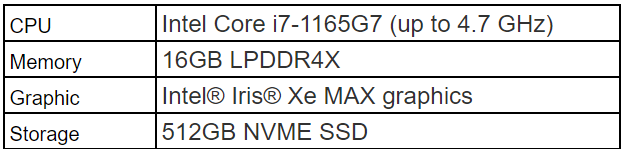
\includegraphics[scale=0.45]{gambar/spek_laptop.png}
  % Keterangan gambar yang diinputkan
  \caption{Spesifikasi Laptop}
  % Label referensi dari gambar yang diinputkan
  \label{fig:spek_laptop}
\end{figure}
Dari sensor kamera yang ada pada drone, penulis akan fokus pada data gambar/video yang dikirimkan ke laptop. Dari data gambar/video itu kemudian didapatkan data kendaraan yang terdeteksi, berupa jenis kendaraan, nilai \emph{confidence}, serta koordinatnya di kamera. Selanjutnya dari data tersebut diekstrak lagi menjadi data antrian kendaraaan yang ada sesuai tujuan penelitian.

\textbf{Peralatan} yang digunakan dalam penelitian ini antara lain:
\begin{enumerate}
  \item \textbf{Laptop} : sebagai perangkat yang berfungsi melakukan penerimaan video, pengolahan video, hingga penampilan hasil akhir dari output yang diharapkan.
  \item \textbf{Drone} : sebagai alat yang berfungsi melakukan pengambilan video di lapangan. Drone yang digunakan harus dilengkapi dengan sensor kamera yang menghadap ke bawah, serta kemampuan untuk mentransmisikan hasil video secara \emph{wireless}.
  \item \textbf{Visual Studio Code} : Digunakan sebagai kode editor, yaitu media untuk menulis dan mengelola kode program, termasuk implementasi algoritma pengolahan citra, \emph{deep learning}, serta estimasi antrian kendaraan yang ada.
  \item \textbf{Framework berkaitan} : mencakup berbagai \emph{framework} dan \emph{tool} untuk menunjang proses pengolahan citra, \emph{deep learning}, dan sebagainya. Beberapa yang bisa digunakan antara lain OpenCV, YOLO, dan Roboflow.
\end{enumerate}

% % Contoh penggunaan referensi dari gambar yang diinputkan
% Pada \emph{blueprint} yang tertera di Gambar \ref{fig:Blueprint}. \lipsum[12]

\section{Metode yang digunakan}
Metodologi yang digunakan pada penelitian ini terdiri dari beberapa tahapan seperti yang ditunjukkan pada gambar berikut.
\begin{figure} [H] \centering
  % Nama dari file gambar yang diinputkan
  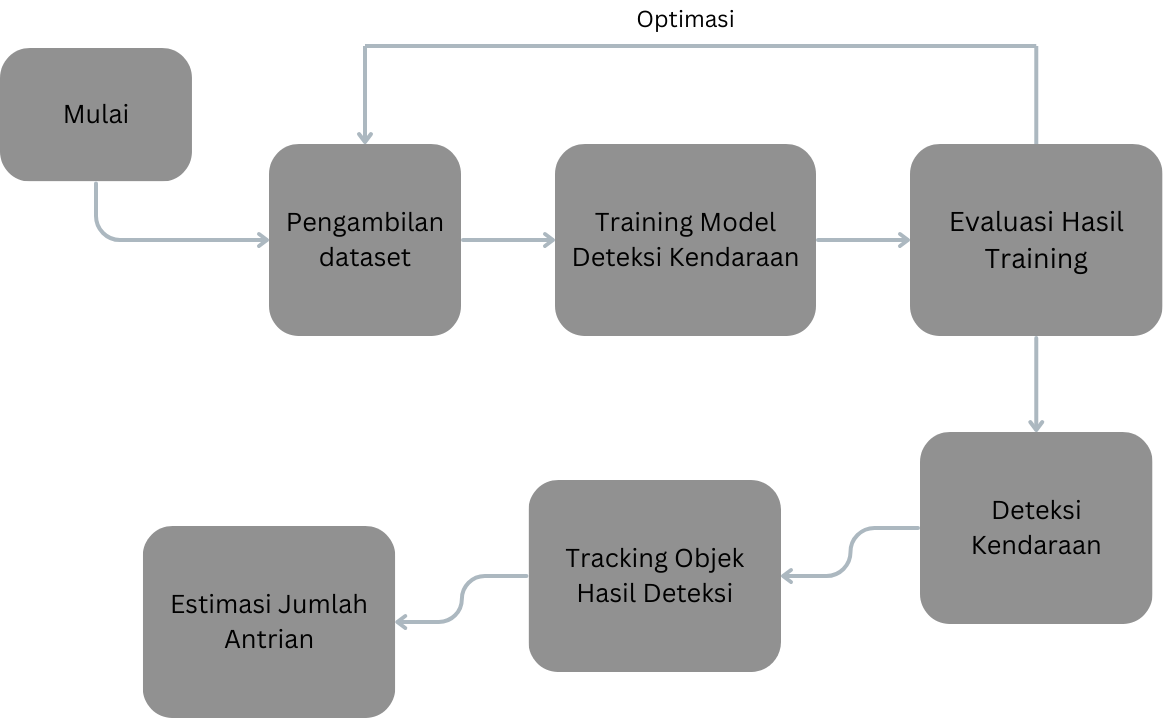
\includegraphics[scale=0.45]{gambar/Blok Diagram Pra-TA NEW.png}
  % Keterangan gambar yang diinputkan
  \caption{Diagram Blok Perancangan Penelitian}
  % Label referensi dari gambar yang diinputkan
  \label{fig:diagaram_blok}
\end{figure}

\subsection{Pengambilan Dataset}
Dataset yang digunakan pada penelitian ini merupakan hasil dari pengambilan gambar keadaan lalu lintas di suatu persimpangan. Pengambilan gambar dilakukan dengan menerbangkan drone pada berbagai ketinggian dan \emph{angle} yang bervariasi. Hal ini dilakukan agar proses training benar-benar menghasilkan model yang akurat.

\subsection{Training Model Deteksi Kendaraan}
Terdapat beberapa prosedur dalam pelaksanaan training model pada penelitian ini.
\begin{figure} [H] \centering
  % Nama dari file gambar yang diinputkan
  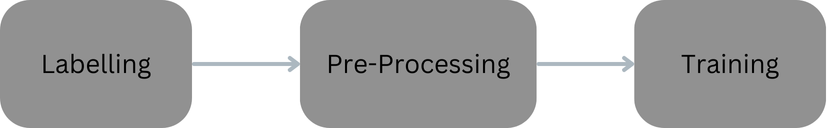
\includegraphics[scale=0.45]{gambar/Blok Diagram Training.png}
  % Keterangan gambar yang diinputkan
  \caption{Diagram Blok Prosedur Training}
  % Label referensi dari gambar yang diinputkan
  \label{fig:diagaram_blok_training}
\end{figure}
Seperti yang ditunjukkan pada \ref{fig:diagaram_blok_training}, awalnya dilakukan proses pelabelan dataset untuk menentukan kelas-kelas objek yang akan dideteksi nantinya. \emph{Pre-Processing} dilakukan dengan mengubah dataset agar sesuai dengan gambar yang digunakan oleh model \emph{object detection}. Perubahan-perubahan tersebut meliputi ukuran gambar yang menjadi lebih kecil dan format gambar serta warna yang disesuaikan dengan yang digunakan oleh model \emph{object detection}. Selanjutnya, model pun dilakukan proses training menggunakan dataset yang sudah siap tersebut.
\begin{figure} [H] \centering
  % Nama dari file gambar yang diinputkan
  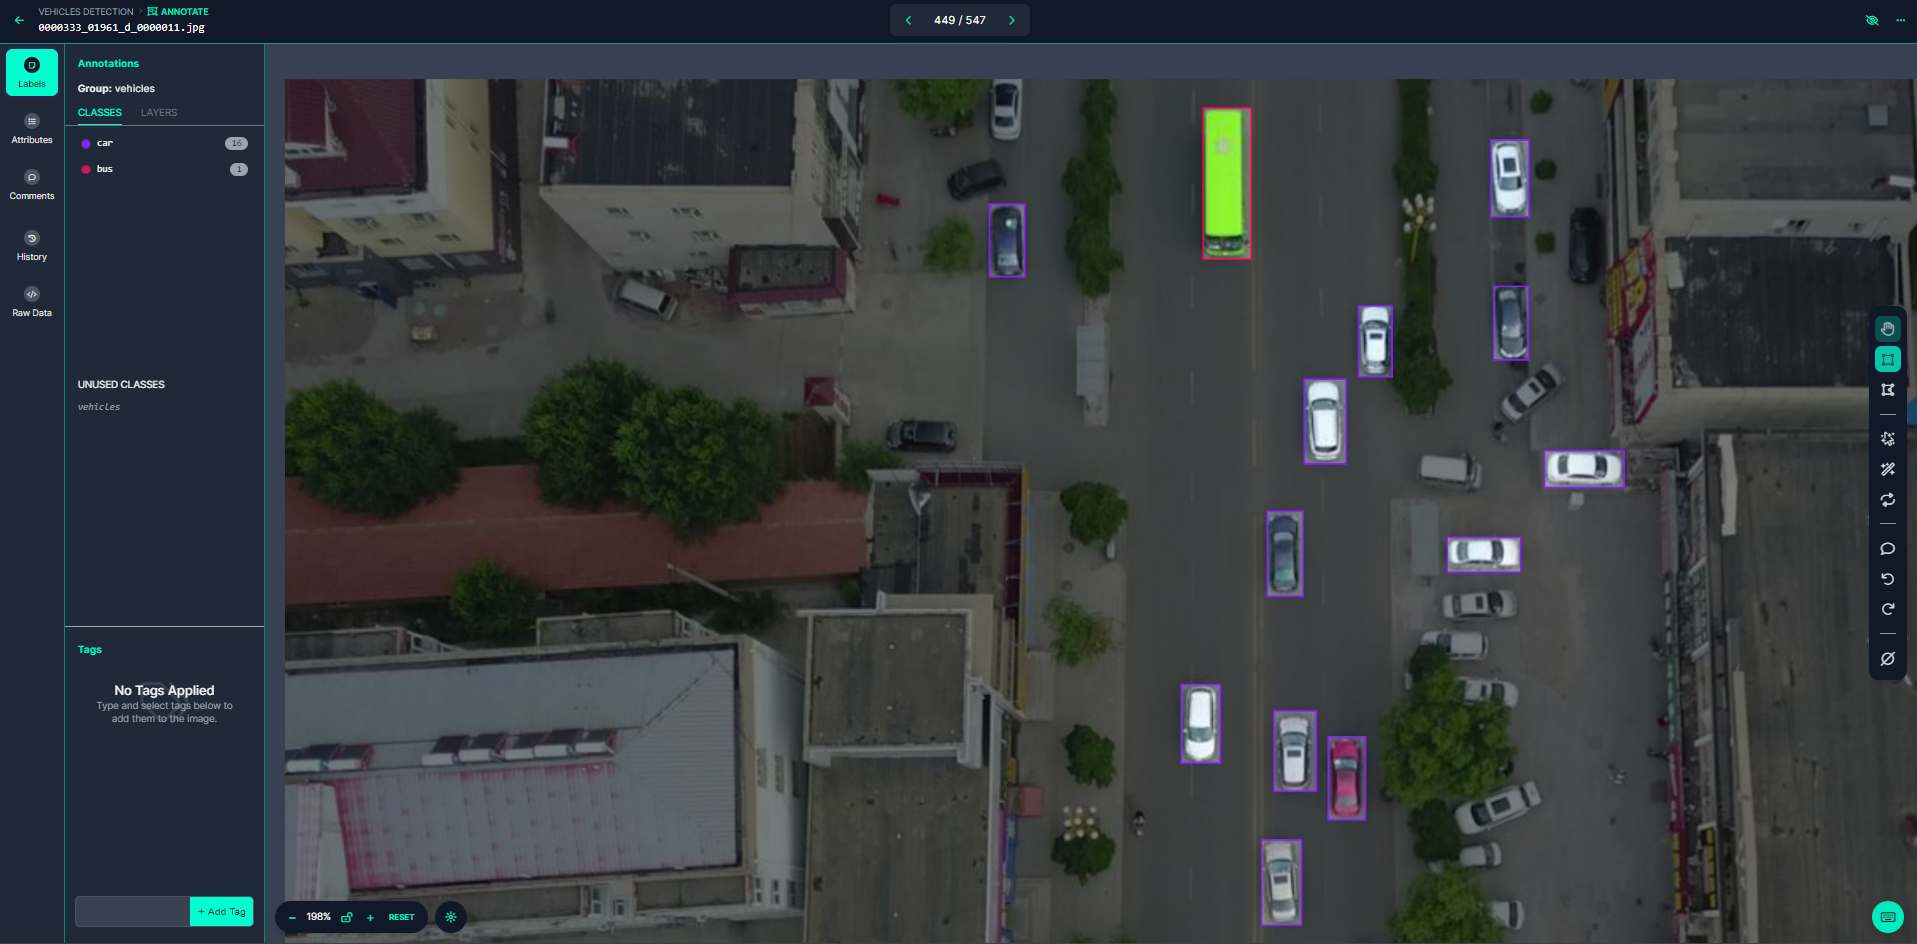
\includegraphics[scale=0.3]{gambar/pelabelan.png}
  % Keterangan gambar yang diinputkan
  \caption{Proses pelabelan dataset}
  % Label referensi dari gambar yang diinputkan
  \label{fig:pelabelan}
\end{figure}

\subsection{Evaluasi Hasil Training}
Proses evaluasi dilakukan dengan melakukan pengetesan terhadap hasil training model. Apabila performa model belum memenuhi ekspektasi, model akan terus ditraining ulang hingga didapatkan hasil performa model yang akurat.

\subsection{Deteksi Kendaraan}
Pada tahap ini, dilakukan proses deteksi menggunakan model yang telah dilatih sebelumnya. Dalam hal ini, objek yang terdeteksi akan diberi \emph{bounding box}, yaitu berupa gambar persegi/kotak yang mengelilingi objek, menandakan model telah berhasil mendeteksi objek yang diinginkan. Terdapat beberapa informasi yang didapatkan saat model berhasil mendeteksi objek, yaitu kelas objek, koordinat objek, serta nilai \emph{confidence} dari hasil deteksi objek. Nilai \emph{confidence} menandakan seberapa yakin model \emph{object detection} berhasil mendeteksi, apabila nilai \emph{confidence} kecil berarti model tidak sebegitu yakin dengan hasil deteksi, begitu pula sebaliknya. Informasi-informasi ini nantinya akan berguna dalam pengolahan data yang lebih lanjut.
\begin{figure} [H] \centering
  % Nama dari file gambar yang diinputkan
  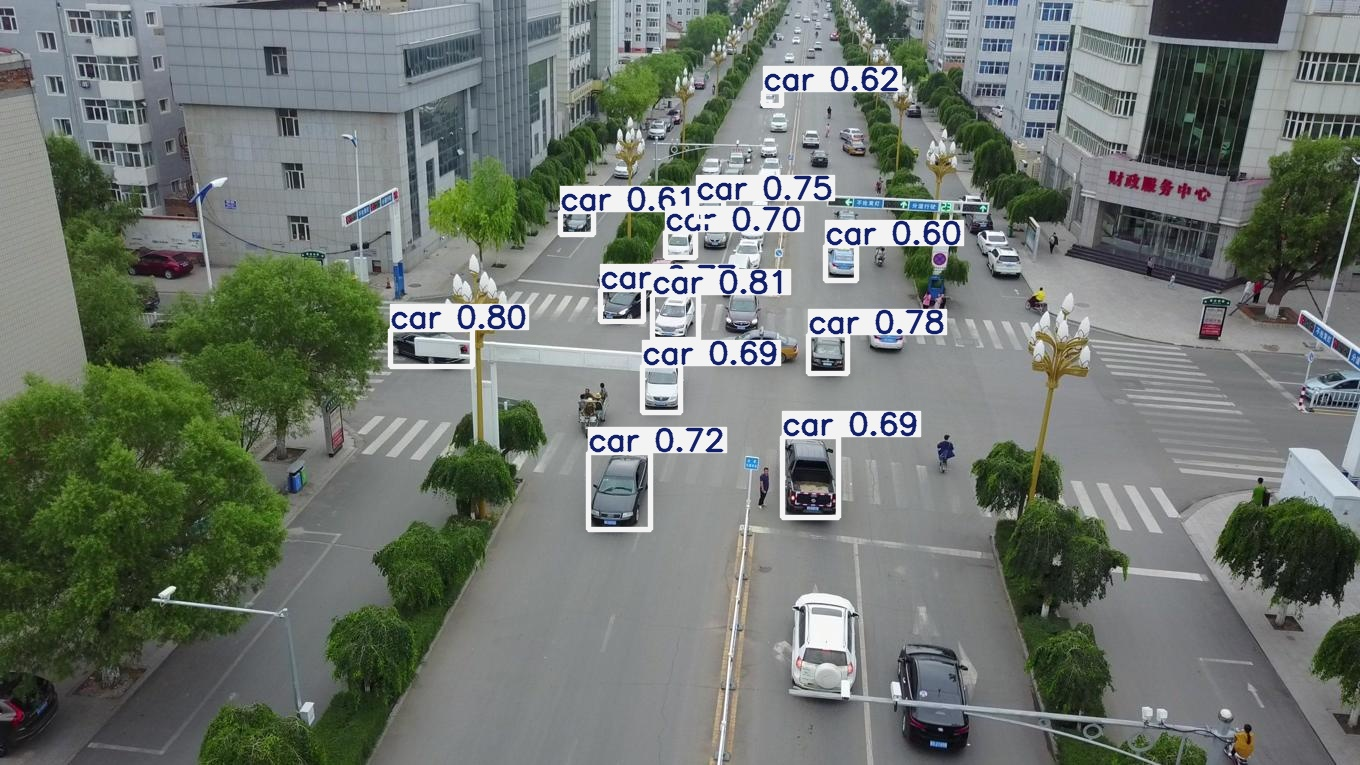
\includegraphics[scale=0.3]{gambar/coco_1.jpg}
  % Keterangan gambar yang diinputkan
  \caption{Proses Deteksi Kendaraan}
  % Label referensi dari gambar yang diinputkan
  \label{fig:deteksi_kendaraan}
\end{figure}

\subsection{\emph{Tracking} Objek Hasil Deteksi}
Pada tahap ini, dilakukan proses \emph{tracking} kendaraan-kendaraan yang sudah dideteksi. Hal ini dapat dilakukan dengan konsep \emph{optical flow}, yaitu mendeteksi pergerakan objek antara dua gambar berturut-turut atau dalam aliran video. Proses ini perlu dilakukan karena penelitian ini bertujuan menghitung antrian kendaraan yang ada di persimpangan lalu lintas, yang mana informasi terkait arah yang dituju oleh suatu kendaraan menjadi hal yang penting. Tentunya algoritma yang disusun harus dapat membedakan antara kendaraan yang sedang berada dalam antrian dengan kendaraan yang tidak.

\subsection{Estimasi Jumlah Antrian Kendaraan}
Maka selanjutnya dilakukan perkiraan atau estimasi mengenai jumlah antrian yang ada pada persimpangan lalu lintas. Proses ini dapat dilakukan dengan pengolahan citra, salah satunya dengan menentukan \emph{region of interest} (ROI). Dengan konsep ini, maka daerah yang tertangkap kamera dapat dipisahkan sehingga akan membantu dalam melakukan estimasi antrian kendaraan yang ada.

\section{Jadwal Penelitian}
Berikut merupakan rencana jadwal pelaksanaan penelitian ini.

% Ubah tabel berikut sesuai dengan isi dari rencana kerja
\newcommand{\w}{}
\newcommand{\G}{\cellcolor{gray}}
\begin{table}[H]
  \captionof{table}{Tabel timeline}
  \label{tbl:timeline}
  \begin{tabular}{|p{3.5cm}|c|c|c|c|c|c|c|c|c|c|c|c|c|c|c|c|}

    \hline
    \multirow{2}{*}{Kegiatan} & \multicolumn{16}{|c|}{Minggu}                                                                       \\
    \cline{2-17}              &
    1                         & 2                             & 3  & 4  & 5  & 6  & 7  & 8  & 9  & 10 & 11 & 12 & 13 & 14 & 15 & 16 \\
    \hline

    % Gunakan \G untuk mengisi sel dan \w untuk mengosongkan sel
    Pengambilan dataset          &
    \G                        & \G                            & \G & \w & \w & \w & \w & \w & \w & \w & \w & \w & \w & \w & \w & \w \\
    \hline

    Training dan evaluasi dataset &
    \w                        & \w                            & \w & \G & \G & \G & \G & \w & \w & \w & \w & \w & \w & \w & \w & \w \\
    \hline

    Deteksi kendaraan         &
    \w                        & \w                            & \w & \w & \w & \w & \G & \G & \G & \w & \w & \w & \w & \w & \w & \w \\
    \hline

    Tracking dan Estimasi Antrian &
    \w                        & \w                            & \w & \w & \w & \w & \w & \w & \w & \G & \G & \G & \G & \G & \w & \w \\
    \hline

    Penyusunan Buku           &
    \w                        & \w                            & \w & \w & \w & \w & \w & \w & \w & \w & \w & \w & \w & \w & \G & \G \\
    \hline
  \end{tabular}
\end{table}

Pada \emph{timeline} yang tertera di Tabel \ref{tbl:timeline}, digambarkan perkiraan jenis kegiatan yang akan dilakukan selama 16 minggu waktu perkuliahan. Diharapakan dengan pembagian yang jelas di awal, dapat menjadi pemandu bagi penulis dalam melaksanakan serta menyelesaikan penelitian dengan baik.

Pada minggu 1 sampai 3, dilakukan pengambilan dataset yang akan digunakan untuk training model. Estimasi durasi ini juga diperkirakan mencakup waktu setup drone untuk bisa terbang mengambil data yang diperlukan. Minggu 4 hingga 7 digunakan untuk melakukan pengolahan dataset yang didapatkan. Pengolahan ini dalam bentuk melakukan pelabelan, augmentasi, training, hingga evaluasi model yang dihasilkan. Rangkaian kegiatan tersebut akan terus diulang-ulang sampai didapatkan model yang akurat, namun juga cukup ringan untuk dijalankan di laptop penulis.

Pada minggu 7 sampai 9, mulai dilakukan percobaan deteksi kendaraan pada lingkungan yang sebenarnya. Selanjutnya pada minggu 10 hingga 14, dilakukan implementasi algoritma untuk proses \emph{tracking} kendaraan serta estimasi jumlah antrian yang ada. Akhirnya, minggu 15 dan 16 merupakan proses penyusunan hasil buku tugas akhir.